\documentclass[12pt]{beamer}

\mode<presentation>{\usetheme{Warsaw}}
\setbeamertemplate{footline}[frame number]
\usepackage[english]{babel}
\usepackage{times}
\usepackage{url}
\usepackage{graphicx}
\usepackage{listings}
\lstloadlanguages{Python}
\lstset{language=Python}
\lstset{%
	basicstyle=\ttfamily\bfseries,
	keywordstyle=\color{blue}, emph={self}, emphstyle={\color{blue}},
	identifierstyle=,
	commentstyle=\color{gray},
	stringstyle=\color{green!50!black},
	showstringspaces=false,
	emph={[2]__init__,__str__}, emphstyle={[2]\color{purple}},
}
\newcommand{\key}[1]{{\color{blue}#1}}
\newcommand{\cmnt}[1]{{\color{gray}#1}}
\newcommand{\str}[1]{{\color{green!50!black}#1}}
\newcommand{\defn}[1]{{\color{purple}#1}}
\newcommand{\SC}[1]{\mbox{\sc#1}}

\title{Adversarial Search}
\subtitle{Introduction to Artificial Intelligence}
\author{Steven Bethard}
\institute{
  Department of Computer Science\\
  University of Colorado
}
\date{CSCI 3202}

\AtBeginSection[]{
  \begin{frame}<beamer>{Outline}
    \tableofcontents[currentsection]
  \end{frame}
}
\begin{document}

\begin{frame}
  \titlepage
\end{frame}

\begin{frame}{Important Dates}
	\begin{block}{Homework: Search}
		Due Thursday September 25, 12:30pm
	\end{block}
	\begin{block}{Quiz: Search}
		Tuesday September 30, 12:30-1:00pm
	\end{block}
\end{frame}
\begin{frame}[fragile]{Comparing Objects in Python}
	\begin{semiverbatim}\scriptsize\bfseries
		>>> \key{class} \defn{Node}(object):
		...     \key{def} \defn{__init__}(\key{self}, score):
		...         \key{self}.score = score
		... \pause
		>>> n2 = Node(2)
		>>> n1 = Node(1)
		>>> n2 < n1\pause
		\key{True}\pause
		>>> \key{class} \defn{Node}(object):
		...     \key{def} \defn{__init__}(\key{self}, score):
		...         \key{self}.score = score
		...     \key{def} \defn{__cmp__}(\key{self}, other):
		...         \key{return} cmp(\key{self}.score, other.score)
		... \pause
		>>> n2 = Node(2)
		>>> n1 = Node(1)
		>>> n2 < n1\pause
		\key{False}
	\end{semiverbatim}
\end{frame}
\begin{frame}[fragile]{Using the \texttt{heapq} Module}
	\begin{semiverbatim}\scriptsize\bfseries
		>>> \key{class} \defn{Node}(object):
		...     \key{def} \defn{__init__}(\key{self}, score):
		...         \key{self}.score = score
		...     \key{def} \defn{__cmp__}(\key{self}, other):
		...         \key{return} cmp(\key{self}.score, other.score)
		... \pause
		>>> \key{import} heapq
		>>> queue = []
		>>> heapq.heappush(queue, Node(3))
		>>> heapq.heappush(queue, Node(7))
		>>> heapq.heappush(queue, Node(1))
		>>> heapq.heappush(queue, Node(5))\pause
		>>> \key{while} queue:
		...         \key{print} heapq.heappop(queue).score
		... \pause
		1
		3
		5
		7
	\end{semiverbatim}
\end{frame}
\begin{frame}[fragile]{Mazes with no Solution}
	\begin{columns}
		\begin{column}{1.5in}
			\begin{semiverbatim}\bfseries\huge
				######
				#\alt<3>{\alert{+}}{ }\alt<3>{\alert{+}}{ }\alt<3>{\alert{+}}{ }##
				#\alt<3>{\alert{+}}{ }## #
				#\key{S}\alt<3>{\alert{+}}{ }#\key{G}#
				######
			\end{semiverbatim}
		\end{column}
		\begin{column}{2.5in}
			\begin{block}{Expected Result}
				\pause
				\begin{itemize}
					\item All reachable squares visited
					\item No path to solution
				\end{itemize}
			\end{block}
		\end{column}
	\end{columns}
\end{frame}

\begin{frame}{Outline}
  \tableofcontents
\end{frame}

\section{Describing Games}
\subsection{Games as Search}
\begin{frame}{Games as Search}
	\begin{block}{Games as Search}
		\begin{description}
			\item[Initial] A board position and which player is to move
			\item[Actions] Moves and resulting states
			\item[Goal] A terminal state, where the game has ended
			\item[Score] Based on utility function, e.g. +1 win, -1 lose
		\end{description}
	\end{block}
	\pause
	\begin{block}{Game Types}
		\centering
		\begin{tabular}{|l|l|l|}
			\hline
			                    & \key{deterministic}               & \key{stochastic} \\
			\hline
			\key{perfect}       & \uncover<3->{chess, checkers,}     & \uncover<4->{backgammon,} \\
			\key{information}   & \uncover<3->{go, othello}          & \uncover<4->{monopoly} \\
			\hline
			\key{imperfect}     & \uncover<5->{battleship,}          & \uncover<6->{bridge, poker,} \\
			\key{information}   & \uncover<5->{blind tic-tac-toe}    & \uncover<6->{scrabble} \\
			\hline
		\end{tabular}
	\end{block}
\end{frame}
\subsection{Game Search Trees}
\begin{frame}{Tic-Tac-Toe Game Tree}
	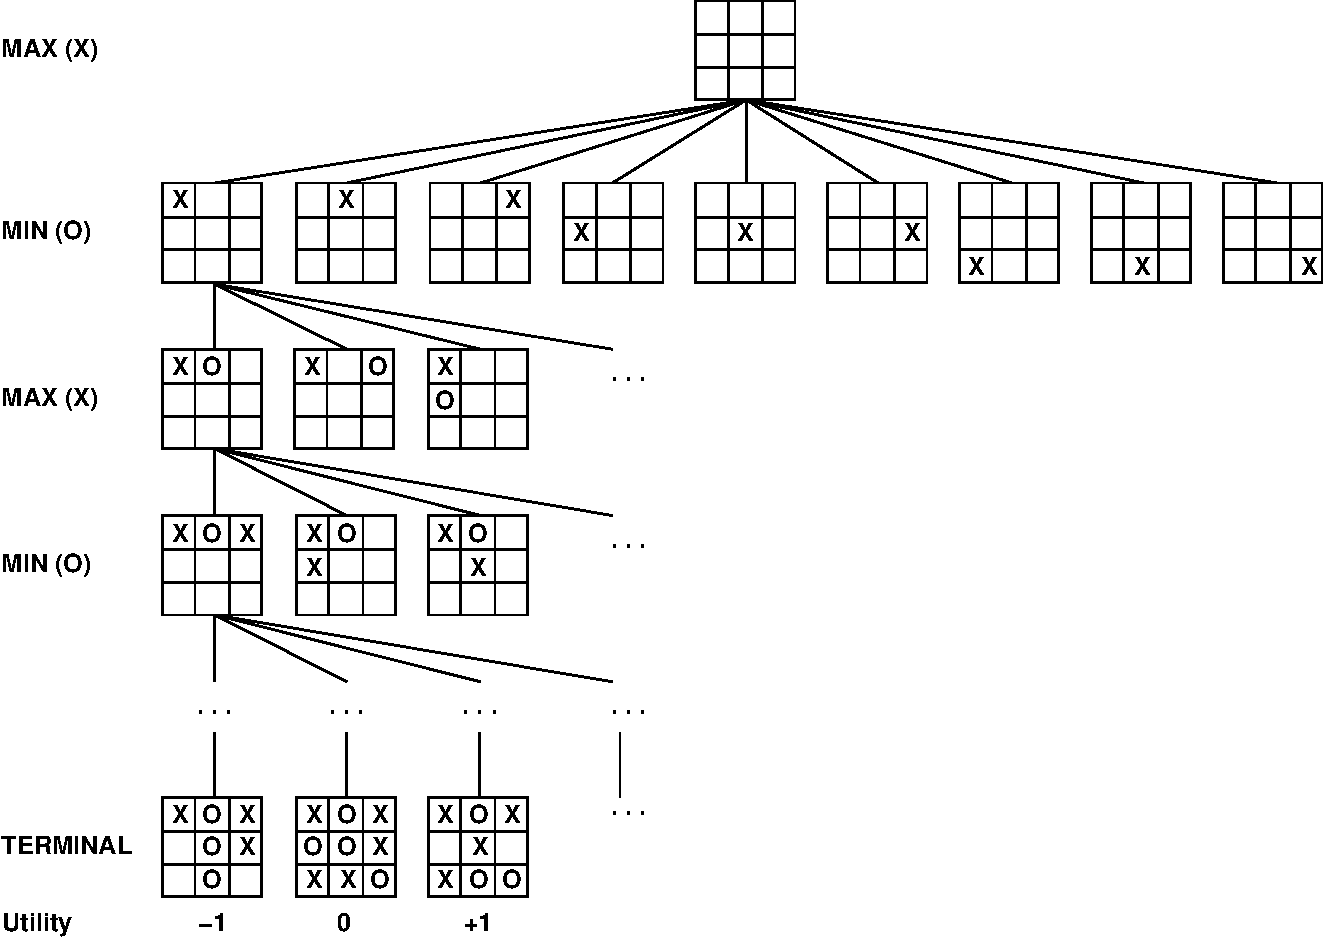
\includegraphics[width=4in]{tictactoe.pdf}
\end{frame}

\section{Deterministic Games}
\subsection{Minimax}
\begin{frame}{Minimax}
	\begin{block}{Idea}
		\begin{itemize}
			\item Expect other player to minimize your utility
			\item Choose action that maximizes the minimized utility
		\end{itemize}
	\end{block}
	\begin{center}
		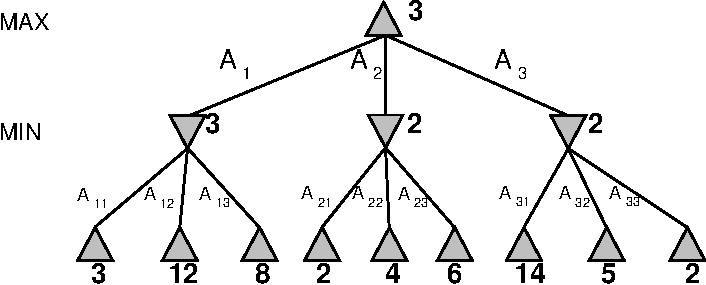
\includegraphics[width=4in]{minimax.pdf}
	\end{center}
\end{frame}
\begin{frame}[fragile]{Minimax Code}
	\begin{semiverbatim}\scriptsize\bfseries
		\key{def} \defn{minimax_decision}(problem, state):
		    \pause\cmnt{# select the action with the maximum utility}
		    value, action = max_value_action(problem, state)
		    \key{return} action
		\pause
		\key{def} \defn{\alt<7>{\alert{min}}{max}_value_action}(problem, state):
		    \pause\cmnt{# simply return the known utility for leaf nodes}
		    \key{if} problem.is_terminal(state):
		        \key{return} problem.get_utility(state), \key{None}
		    \pause\cmnt{# collect utility values for each available action}
		    items = []
		    \key{for} action, state \key{in} problem.get_successors(state):
		        value, _ = \alt<7>{\alert{max}}{min}_value_action(problem, state)
		        items.append((value, action))
		    \pause\cmnt{# return the action with the \alt<7>{\alert{min}}{max}imum utility}
		    \key{return} \alt<7>{\alert{min}}{max}(items)
	\end{semiverbatim}
\end{frame}
\begin{frame}{Minimax Exercise}
	\begin{columns}
		\begin{column}{2in}
			\begin{block}{Build the Minimax Tree}
				\begin{itemize}
					\item It is X's turn
					\item Scoring: \\
						\begin{tabular}{lr}
							\key{X Wins}      & +1 \\
							\key{X Loses}     & -1 \\
							\key{X and O Tie} &  0 \\
						\end{tabular}
				\end{itemize}
			\end{block}
		\end{column}
		\begin{column}{2in}
			\centering\Huge
			\begin{tabular}{c|c|c}
				O & X & X \\
				\hline
				X &   &   \\
				\hline
				O & O &   \\
			\end{tabular}
		\end{column}
	\end{columns}
\end{frame}
\begin{frame}{Minimax Properties}
	\begin{center}
		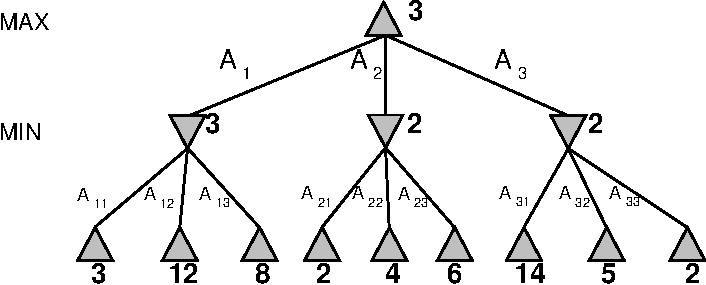
\includegraphics[width=3.5in]{minimax.pdf}
	\end{center}
	\begin{tabular}{ll}
		\key{Complete?} \pause & Yes, if tree is finite \pause \\
		\key{Optimal?}  \pause & Yes, for optimal opponent \pause \alert{and suboptimal!} \pause \\
		\key{Time?}     \pause & $O(b^m)$, all nodes in the tree \pause \\
		\key{Space?}    \pause & $O(bm)$, like depth first search \\
	\end{tabular}
\end{frame}
\begin{frame}{Multiplayer Minimax}
	\begin{block}{Idea}
		Store a tuple of utilities for each node
	\end{block}
	\pause
	\begin{block}{Multiplayer Game Tree}
		\centering
		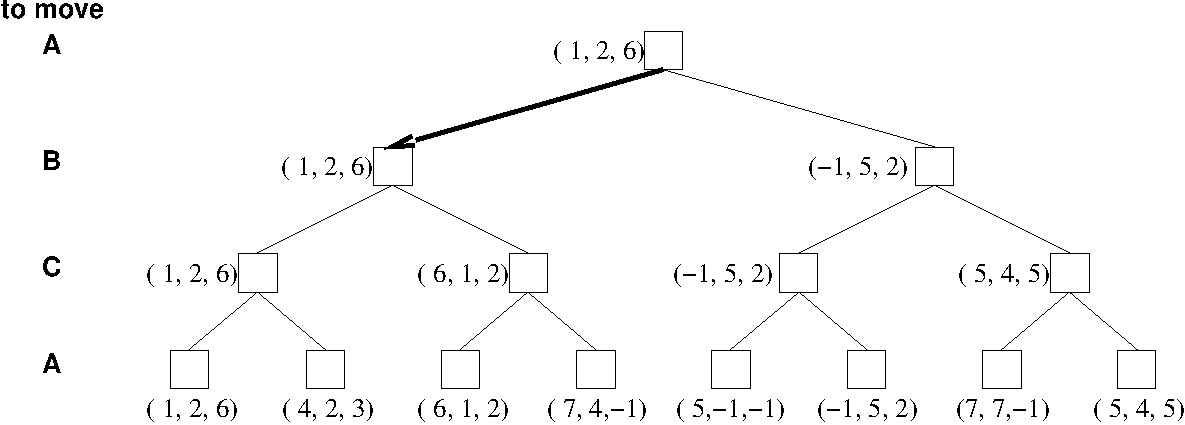
\includegraphics[width=4in]{minimax-multi.pdf}
	\end{block}
\end{frame}

\subsection{Alpha-Beta Pruning}
\begin{frame}{Alpha-Beta Pruning}
	\begin{block}{Idea}
		Skip branches that have no effect on final values
	\end{block}
	\bigskip
	\only<1>{\invisible{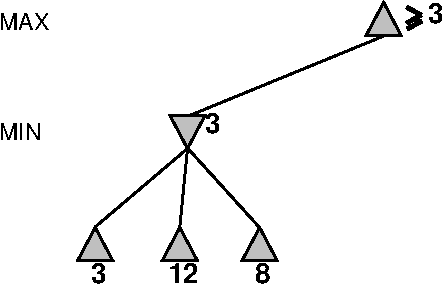
\includegraphics[height=1.5in]{alpha-beta-progress-1.pdf}}}%
	\only<2>{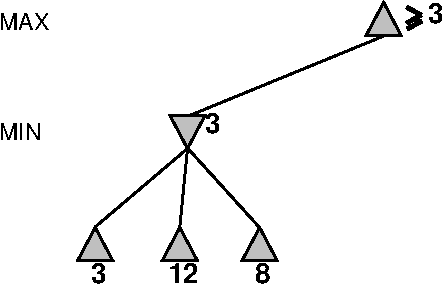
\includegraphics[height=1.5in]{alpha-beta-progress-1.pdf}}%
	\only<3>{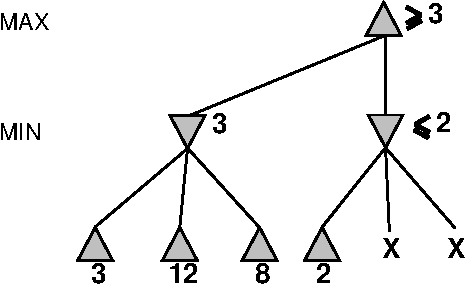
\includegraphics[height=1.5in]{alpha-beta-progress-2.pdf}}%
	\only<4>{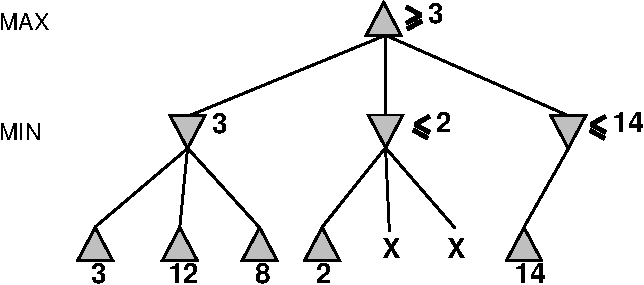
\includegraphics[height=1.5in]{alpha-beta-progress-3.pdf}}%
	\only<5>{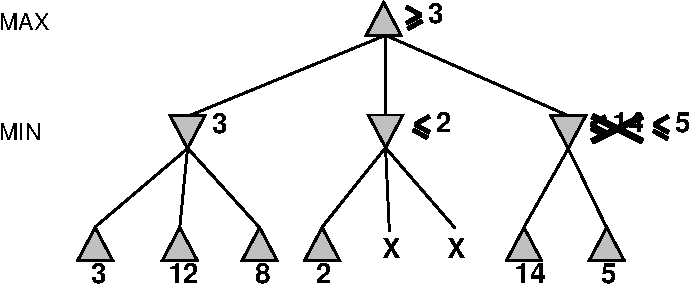
\includegraphics[height=1.5in]{alpha-beta-progress-4.pdf}}%
	\only<6>{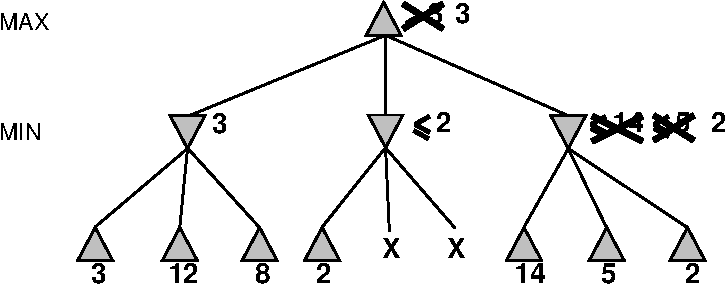
\includegraphics[height=1.5in]{alpha-beta-progress-5.pdf}}%
\end{frame}
\begin{frame}{Alpha-Beta Pruning in General}
	\begin{columns}
		\begin{column}{2in}
			\begin{block}{Idea}
				If $m$ is a better choice, then $n$ will never be reached
			\end{block}
			\begin{block}<2->{Alpha-Beta Bookkeeping}
				\begin{itemize}
					\item[$\alpha$] Best value for Player \\ (the highest value)
					\item[$\beta$] Best value for Opp \\ (the lowest value)
				\end{itemize}
			\end{block}
		\end{column}
		\begin{column}{2in}
			\begin{center}
				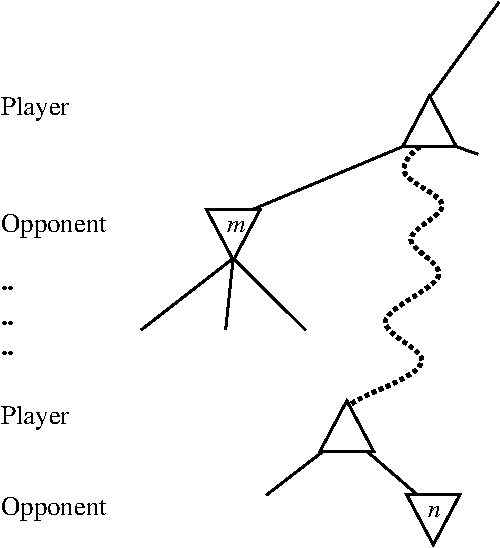
\includegraphics[width=2in]{alpha-beta-general.pdf}
			\end{center}
		\end{column}
	\end{columns}
\end{frame}
\begin{frame}[fragile]{Alpha-Beta Pruning Code}
	\begin{semiverbatim}\scriptsize\bfseries
		\key{def} \defn{alpha_beta_search}(problem, state):
		    \pause\cmnt{# select the action with the maximum utility}
		    value, action = max_ab(state, neg_inf, pos_inf)
		    \key{return} action
		\pause
		\key{def} \defn{\alt<9>{\alert{min}}{max}_ab}(problem, state, alpha, beta):
		    \pause\cmnt{# simply return the known utility for leaf nodes}
		    \key{if} problem.is_terminal(state):
		        \key{return} problem.get_utility(state), \key{None}
		    \pause\cmnt{# examine utility values for each available action}
		    value, action = neg_inf, \key{None}
		    \key{for} action2, state2 \key{in} problem.get_successors(state):
		        value2, _ = \alt<9>{\alert{max}}{min}_ab(problem, state2, alpha, beta)
		        \pause\cmnt{# return the new value if \alt<9>{\alert{lower }}{higher} than the global \alt<9>{\alert{max}}{min}imum}
		        value, action = \alt<9>{\alert{min}}{max}([value, action], [value2, action2])
		        \key{if} value\alt<9>{\alert{ <= alpha}}{ >=  beta}:
		            \key{return} value, action
		        \pause\cmnt{# otherwise, update the global \alt<9>{\alert{min}}{max}imum}
		        \alt<9>{\alert{beta }}{alpha} = \alt<9>{\alert{min}}{max}(\alt<9>{\alert{beta}, }{alpha,} value)
		    \pause\cmnt{# return the action with the \alt<9>{\alert{min}}{max}imum utility}
		    \key{return} value, action
	\end{semiverbatim}
\end{frame}
\begin{frame}{Alpha-Beta Pruning Properties}
	\begin{center}
		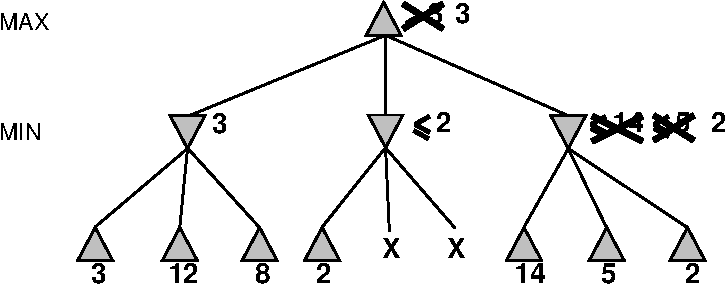
\includegraphics[height=1.5in]{alpha-beta-progress-5.pdf}
	\end{center}
	\begin{block}{Time Complexity}
		\begin{itemize}
			\pause
			\item ``Perfectly'' ordered branches gives $O(b^{m/2})$
			\pause
			\item Still exponential, but doubles solvable depth
		\end{itemize}
	\end{block}
\end{frame}

\subsection{Approximate Solutions}
\begin{frame}[fragile]{Approximate Solutions}
	\begin{block}{Problem}
		Even with Alpha-Beta Pruning, chess space is still $35^{50}$
	\end{block}
	\pause
	\begin{block}{Solution}
		Don't search the entire tree:
		\begin{semiverbatim}\scriptsize\bfseries
		    \key{if} problem.\alt<3->{\alert{is_past_cutoff}}{is_terminal}(state):
		        \key{return} problem.\alt<3->{\alert{get_estimated_utility}}{get_utility}(state)
		
		\end{semiverbatim}
	\end{block}
	\pause\pause
	\begin{block}{Example}
		\begin{itemize}
			\item Given 100 seconds
			\item Given ability to explore $10^4$ nodes/second
			\item Can explore to depth $\approx 8$ ($10^6 \approx 35^{8/2}$)
		\end{itemize}
	\end{block}
\end{frame}
\begin{frame}{Evaluation Functions}
	\begin{block}{Necessary Properties}
		\begin{itemize}
			\item Quickly computable
			\item Orders terminal states by utility
			\item Correlated with chances of winning
		\end{itemize}
	\end{block}
	\pause
	\begin{block}{Typical Approach}
		Weighted linear combination of features:
		\[\mbox{\sc Eval}(s) = w_1 f_1(s) + w_1 f_2(s) + \ldots + w_n f_n(s)\]
	\end{block}
\end{frame}
\begin{frame}{Example Evaluation Function}
	\centering
	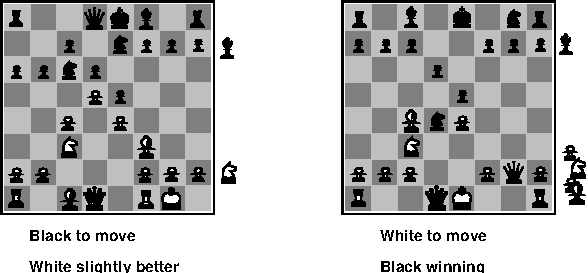
\includegraphics[height=1.75in]{chess-evaluation.pdf}
	\begin{block}{Weighted Features}
		\small
		$
		\begin{array}{rcl}
			w_{\mbox{\scriptsize pawn}}  \cdot f_{\mbox{\scriptsize pawn}}(s)  & = & 1 \cdot (\mbox{white pawns} - \mbox{black pawns})   \\
			\ldots                                                             & = & \ldots \\
			w_{\mbox{\scriptsize queen}} \cdot f_{\mbox{\scriptsize queen}}(s) & = & 9 \cdot (\mbox{white queens} - \mbox{black queens})
		\end{array}
		$
	\end{block}
\end{frame}
\begin{frame}{Deterministic Games in Practice}
	\begin{block}{Checkers}
		\begin{itemize}
			\item\small 1994: Chinook ``Man-Machine World Champion'' (0-0-6)
			\item\small 2007: Chinook's creators ``proved'' it cannot lose
			\item\small End-game database for all $\leq 10$ piece states
		\end{itemize}
	\end{block}
	\begin{block}{Chess}
		\begin{itemize}
			\item\small 1997: Deep Blue defeated Garry Kasparov (2-1-3)
			\item\small 200 million positions per second, searching 6-40 plies
			\item\small End-game database for all $\leq 5$ piece states
		\end{itemize}
	\end{block}
	\begin{block}{Go}
		\begin{itemize}
			\item\small Computers still rank as intermediate amateurs
			\item\small Go has $\approx 150$�-$250$ moves per turn
		\end{itemize}
	\end{block}
\end{frame}

\section{Nondeterministic Games}

\subsection{Describing Nondeterministic Games}
\begin{frame}{Nondeterministic Game: Backgammon}
	\begin{center}
		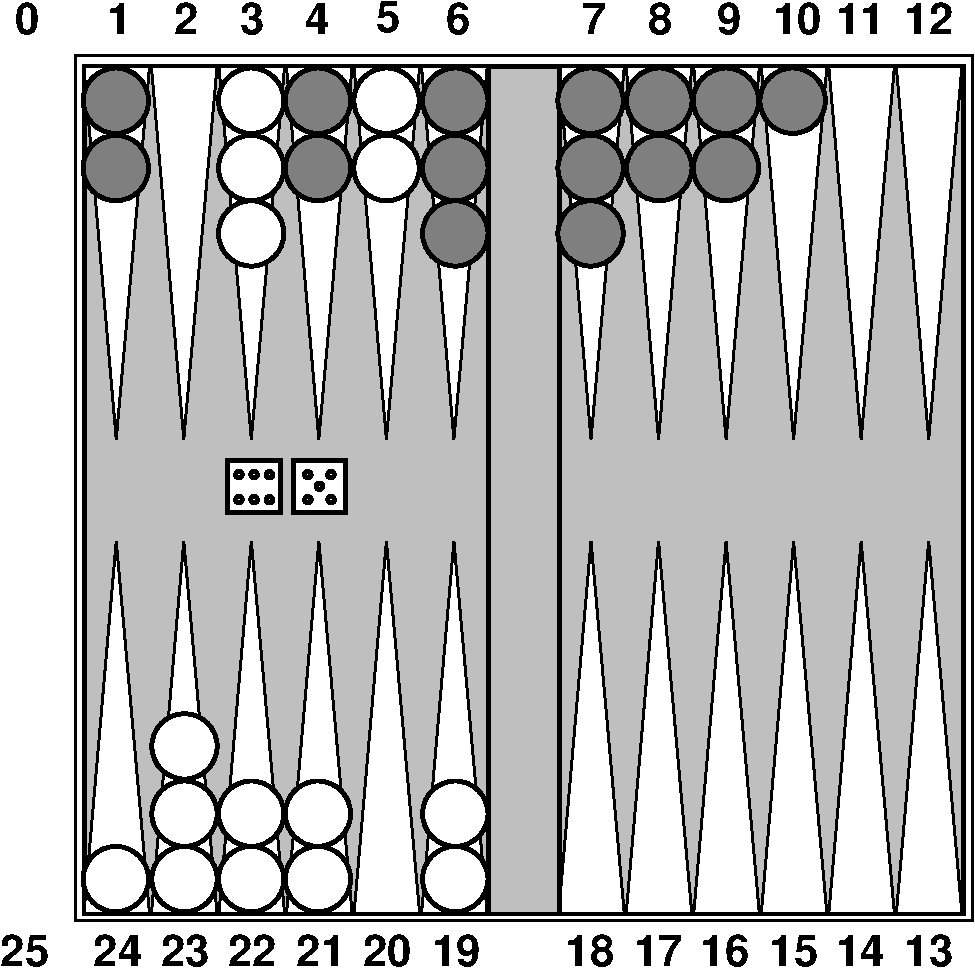
\includegraphics[height=2.5in]{backgammon-position.pdf}
	\end{center}
\end{frame}
\begin{frame}{Backgammon Game Tree}
	\begin{center}
		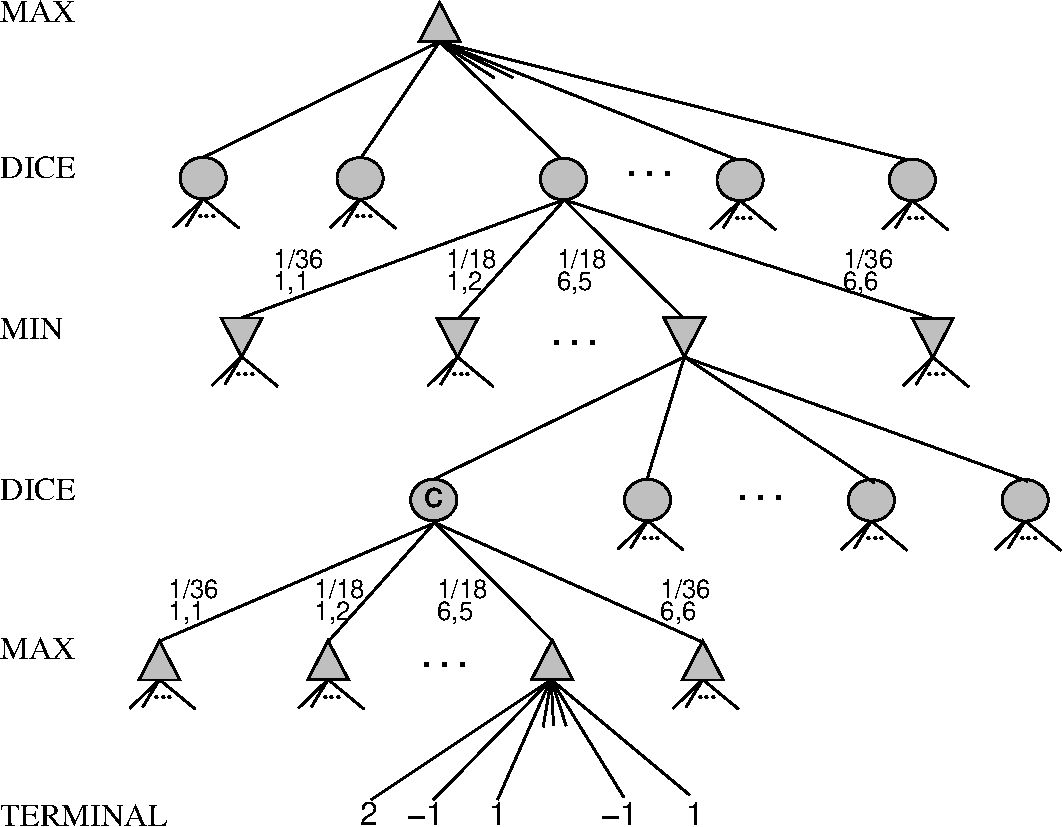
\includegraphics[height=2.5in]{backgammon-tree.pdf}
	\end{center}
\end{frame}

\subsection{Expectiminimax}
\begin{frame}{Expectiminimax}
	\begin{block}{Expected Values for Chance Nodes}
		\[\SC{Expecti}(n) = \sum\limits_{s \in \SC{\scriptsize Successors}(n)}{P(s) \cdot \SC{Expecti}(s)}\]
	\end{block}
	\begin{center}
		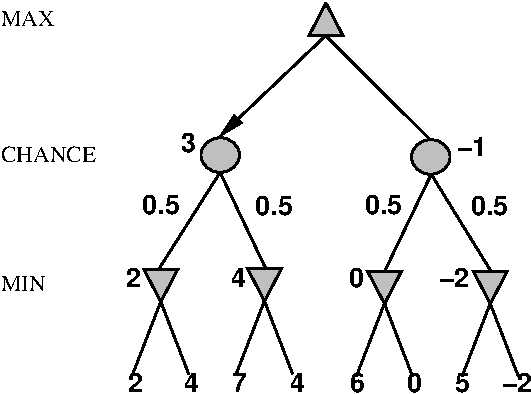
\includegraphics[height=1.75in]{expectiminimax-simple.pdf}
	\end{center}
\end{frame}
\begin{frame}{Expectiminimax Practice}
	\begin{block}{A Simple Game}
		\begin{itemize}
			\item Deck contains J, Q, K, K
			\item One card will be selected by the players
			\item Player 1 draws first, and either:
				\begin{itemize}
					\item Keeps the card and the game is over, or
					\item Removes the card and Player 2 draws and either:
						\begin{itemize}
							\item Keeps the card and the game is over
							\item Discards the card and a final card is drawn
						\end{itemize}
				\end{itemize}
			\item A final J scores -1, Q scores 0, and K scores +1
		\end{itemize}
	\end{block}
\end{frame}
\begin{frame}{Using Expectiminimax}
	\begin{block}{Expectiminimax Properties}
		\begin{tabular}{ll}
			\key{Complete?} \pause & Yes, if tree is finite (both moves and ``rolls'') \pause \\
			\key{Optimal?}  \pause & Yes \pause \\
			\key{Time?}     \pause & $O(b^mn^m)$, all nodes, all ``roll'' sequences \\
		\end{tabular}
	\end{block}
	\pause
	\begin{block}{Consequences}
		\begin{tabular}{ll}
			\key{Branching Factor?}   \pause & Increased by dice rolls \pause \\
			\key{Node Likelihood?}    \pause & Decreases with depth \pause \\
			\key{Alpha-Beta Pruning?} \pause & Effectiveness decreased \\
		\end{tabular}
	\end{block}
	\pause
	\begin{block}{Real-World Example: TD-Gammon}
		\begin{itemize}
			\item Depth-2 search, no Alpha-Beta pruning
			\item Neural network eval function trained by self-play
		\end{itemize}
	\end{block}
\end{frame}
\begin{frame}{Utilities in Expectiminimax}
	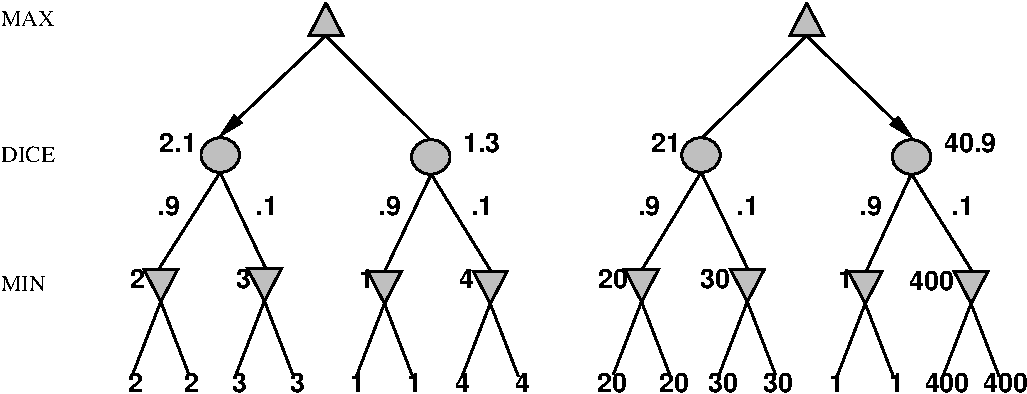
\includegraphics[width=4in]{utility-chance.pdf}
	\pause
	\\ \bigskip
	\begin{block}{Requirement}
		Evaluation function must be a linear transform of utility
	\end{block}
\end{frame}
\begin{frame}{Utilities in Deterministic Games}
	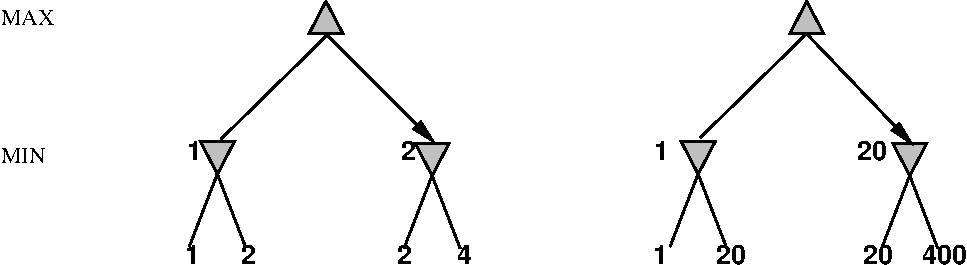
\includegraphics[width=4in]{utility-deterministic.pdf}
	\pause
	\\ \bigskip
	\begin{block}{Requirement}
		Evaluation function need only match the utility ordering
	\end{block}
\end{frame}

\subsection{Games with Imperfect Information}
\begin{frame}[t]{Imperfect Information: Bridge}
	\bigskip
	\only<1>{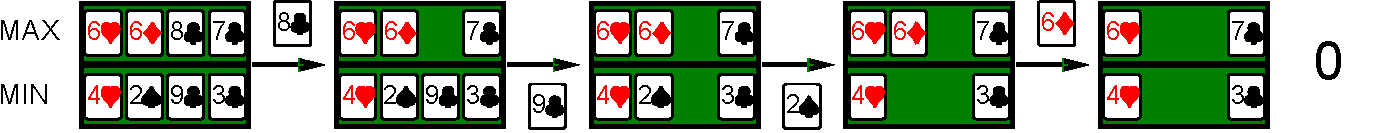
\includegraphics[width=4.2in]{card-tree-1.pdf}}%
	\only<2>{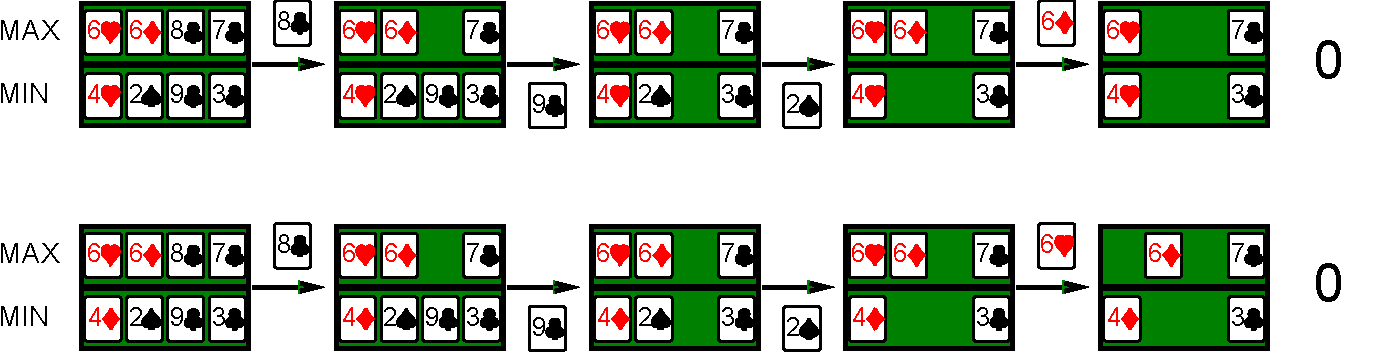
\includegraphics[width=4.2in]{card-tree-2.pdf}}%
	\only<3>{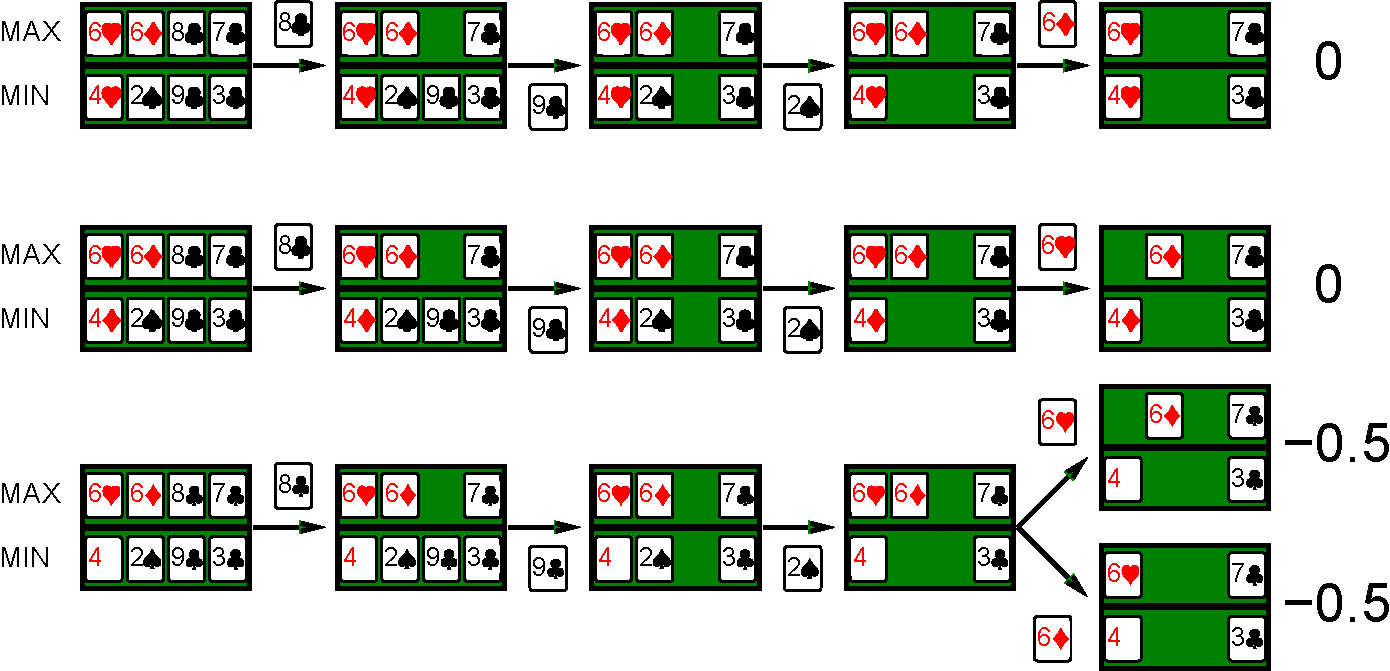
\includegraphics[width=4.2in]{card-tree-3.pdf}}%
\end{frame}
\begin{frame}{Imperfect Information: Common Sense}
	\begin{itemize}
		\item Road A leads to a small heap of gold pieces
		\item \alert<2->{Road B} leads to a fork:
			\begin{itemize}
				\item Take the \alert<2->{left fork} and you'll find a mound of jewels
				\item Take the right fork and you'll be run over by a bus
			\end{itemize}
	\end{itemize}
	\begin{itemize}
		\item<3-> Road A leads to a small heap of gold pieces
		\item<3-> \alert<4->{Road B} leads to a fork:
			\begin{itemize}
				\item<3-> Take the left fork and you'll be run over by a bus
				\item<3-> Take the \alert<4->{right fork} and you'll find a mound of jewels
			\end{itemize}
	\end{itemize}
	\begin{itemize}
		\item<5-> \alert<6->{Road A} leads to a small heap of gold pieces
		\item<5-> Road B leads to a fork:
			\begin{itemize}
				\item<5-> Guess correctly and you'll find a mound of jewels
				\item<5-> Guess incorrectly and you'll be run over by a bus
			\end{itemize}
	\end{itemize}
\end{frame}
\begin{frame}{Imperfect Information}
	\begin{block}{Key Point}
		Value of an action \alert{is not} the average across all states \\
		\pause
		Should be searching through a tree of \alert{belief} states, and:
		\begin{itemize}
			\item Acting to obtain information
			\item Signalling to one's partner
			\item Acting randomly to minimize information disclosure
		\end{itemize}
	\end{block}
	\pause
	\begin{block}{But in the Real World\ldots}
		Most programs use Monte-Carlo estimation:
		\begin{itemize}
			\item Generate 100+ deals consistent with bidding
			\item Pick action that wins most tricks on average
		\end{itemize}
	\end{block}
\end{frame}

\part{Key Points}
\begin{frame}{Key Points}
	\begin{block}{Representing Games}
		\begin{itemize}
			\item Multiple plies per round, one per player
			\item Stochastic games introduce chance nodes
		\end{itemize}
	\end{block}
	\begin{block}{Optimal Solutions}
		\begin{itemize}
			\item (Expecti-)Minimax produces optimal actions
			\item Search belief states when information is incomplete
		\end{itemize}
	\end{block}
	\begin{block}{Approximate Solutions}
		\begin{itemize}
			\item (Expecti-)Minimax explores the whole tree
			\item Approximations use utility estimates and cutoffs
			\item Chance dramatically reduces the depth explored
		\end{itemize}
	\end{block}
\end{frame}

\end{document}


